\chapter{Analyse}

Ziel dieser Arbeit ist es, ein Modell zu entwickeln, das es ermöglicht große Mengen von Bildern zu gruppieren. Wegen der großen Mengen an Daten, die zu verarbeiten sind, sollen \textit{state of the art} Verfahren genutzt werden, die speziell hierauf ausgelegt sind. Der erste der Teil der Analyse befasst sich daher mit dem Bereich des \textit{Machine Learning}. Hier handelt es sich um keine umfängliche Einführung. Es werden Methoden beleuchtet, die zur Komprimierung und Gruppierung von Daten dienen und die Basis des hier vorgeschlagenen Modells bilden. Anhand der Anforderungen und Annahmen wird dann ein unüberwachtes Lernverfahren ausgewählt, dass zu Gruppierung von Bildern dient und in den folgenden Kapiteln weiter ausgearbeitet und realisiert wird. \newline
Im zweiten Teil sollen Möglichkeiten untersucht werden, aus Bildern Features zu gewinnen, welche als Eingabe für das Modell dienen. Um einen Überblick über Features in der Bildverarbeitung zu gewinnen, werden zunächst einige Feature-Detektoren bzw. Deskriptoren für unterschiedlicher Anwendungsfälle angeführt. Heute ist es kaum vorstellbar, dass ein Feature-Deskriptor jeden möglichen Anwendungsfall abdecken kann. Daher soll abschließend der Fokus dieser Arbeit festgelegt werden: Sollen beispielsweise Gesichter oder Szenen erkannt werden? Sollen Objekte erkannt werden und wenn ja, beliebige Kategorien? Anhand der gewonnen Erkenntnisse wird dann entschieden, welche Eigenschaften der hier verwendete Feature-Deskriptor aufweisen soll. 

\section{Verwendung der GPU}

Zum Aufbauen eines Modells werden mehrere Zehn- bis Hunderttausend Features verarbeitet werden. Viele der Verfahren, die der Erzeugung solcher Modellen zu Grunde liegen, wurden in den vergangenen Jahren durch die Verwendung der GPU statt der CPU beschleunigt. Bei der Betrachtung geeigneter Ansätze wird daher auch berücksichtigt, ob und wie eine Beschleunigung durch parallele Verarbeitung erzielt werden kann. Gerade bei großen Datenmengen und einer enormen Datenparallelität können Probleme durch GPUs um ein vielfaches schneller gelöst werden als durch CPUs. Da Nvidias CUDA an der Hochschule Hannover sowohl gelehrt als auch zu Forschungszwecken genutzt wird und sich CUDA auch international in Forschung und Wirtschaft etabliert hat, soll die Plattform als technische Basis dienen. 

\section{Geeignete unüberwachte Lernverfahren}

Für die Gruppierung des Bildmaterials eignen sich maschinelle Lernverfahren besonders, da sie zum einen auf eine große Menge an Trainingsdaten angewiesen sind, um ein nützliches Modell zu generieren und zum anderen eine parallele Verarbeitung begünstigen. Der Einsatz unüberwachter Lernverfahren ist hier aus folgenden Gründen plausibel:

\begin{itemize}
	\item Das Gruppieren bzw. Kategorisieren von Daten ist ein Teilgebiet der unüberwachten Lernverfahren. Hier wird von Clustering gesprochen.
	\item Die Feature-Vektoren umfassen oft viele Komponenten, welche zur Kodierung der Eigenschaften erforderlich sind. Unüberwachte Lernalgorithmen ermöglichen ein exploratives Vorgehen: Die Feature-Vektoren werden auf ihre wesentlichen Komponenten analysiert und so eine kompaktere Darstellung erzeugt.
	\item Es sollen Strukturen in den Daten entdeckt werden, die nicht a priori bekannt sind. Ein überwachter Ansatz erfordert zum Training \textit{gelabelte} Daten, um Vorhersagen zu treffen. Da die gesuchten Strukturen aber gerade nicht bekannt sind, scheidet ein überwachter Ansatz aus.
\end{itemize}

Das Gruppieren von Vektoren, hier den Bild-Features, kann also durch einen \textit{Clustering} Algorithmus umgesetzt werden. Außerdem scheint es sinnvoll die Features vor dem Clustering aufzubereiten: Durch eine kompaktere Darstellung der Vektoren kann der notwendige Speicher reduziert und die Berechnung beschleunigt werden. Nach dem Clustering folgt daher eine Übersicht über den Bereich sogenannter assoziativer Verfahren: Hier werden Strukturen in den Daten gesucht, die nicht offensichtlich sind. Durch die Verwendung dieser unterliegenden Strukturen kann auf einen Teil der ursprünglichen Information verzichtet werden. Da hieraus Vektoren mit weniger Komponenten resultieren, wird auch von \textit{dimensionality reduction} gesprochen.

\textbf{Clustering-Verfahren} quantisieren die Daten in Gruppen. Eine Gruppe steht hier für ein semantisches Merkmal und vertritt eine Menge von konkreten Daten. Unter Clustering-Verfahren fallen Algorithmen wie k-means, hierarchical clustering oder etwa das Gaussian Mixture Model.\newline
Ein Clustering-Algorithmus hat in dem Kontext dieser Arbeit das Ziel, eine großen Menge Feature-Deskriptoren auf die Wesentlichen zu reduzieren. Durch diese Quantisierung in $n$ Gruppen müssen, bei einer Bewertung eines neuen Deskriptors, nur $n$ Deskriptoren betrachtet werden, statt jedes Deskriptors der Ursprungsmenge.\newline
Um die Features zu gruppieren, soll ein k-means Clustering-Verfahren verwendet werden. Anhand der durch k-means gewonnenen Cluster kann eine Histogrammdarstellung für Features erzeugt werden. Die Kombination dieser Verfahren wird Bag of Visual Words genannt und lehnt sich an das Bag of Words-Modell an. K-means ist einer der einfachsten Vertreter der Clustering-Algorithmen, doch die Adaptierung zur Ausführung auf Grafikkarten bringt eine hohe technische Komplexität mit (Speicherverwaltung auf \textit{host} und \textit{device}, Wahl der Blockdimension, Threadanzahl etc.). Bevor also ein anspruchsvollerer Clustering-Algorithmus in Betracht gezogen wird, soll zunächst die Realisierung des k-means-Algorithmus gelingen. Das parallele Verarbeiten von Histogrammen ist ein Lehrbuchbeispiel für den Einsatz von Grafikkarten, da es durch parallele Reduzierung, ein Muster für einige Probleme, erreicht werden kann.

\textbf{Verfahren zu Reduzierung der Dimensionalität} nehmen an, dass es eine unterliegende Struktur gibt, welche entdeckt werden kann. Ein Vektor aus einem $n$-dimensionalen Raum wird auf einen $m$-dimensionalen Raum mit $m < n$ abgebildet. Um die Grundidee zu vermitteln, soll ein einfaches Beispiel dienen: Die roten Punkte in Abbildung \ref{img:compress2} stellen Messwerte dar. Durch die eingezeichnete Linie wird deutlich, dass die Funktion $f(x)=2y$ die Verteilung sehr gut annähert. Würden diese Werte beispielsweise über ein Netzwerk übertragen, so reicht es $x$ zu senden. Der Empfänger kann dann $y$ anhand der Funktion bestimmen. Dadurch könnte 50\% der Daten bei der Übertragung eingespart werden und nur wenig Information geht verloren.\newline 
\begin{figure}
	\centering
	
	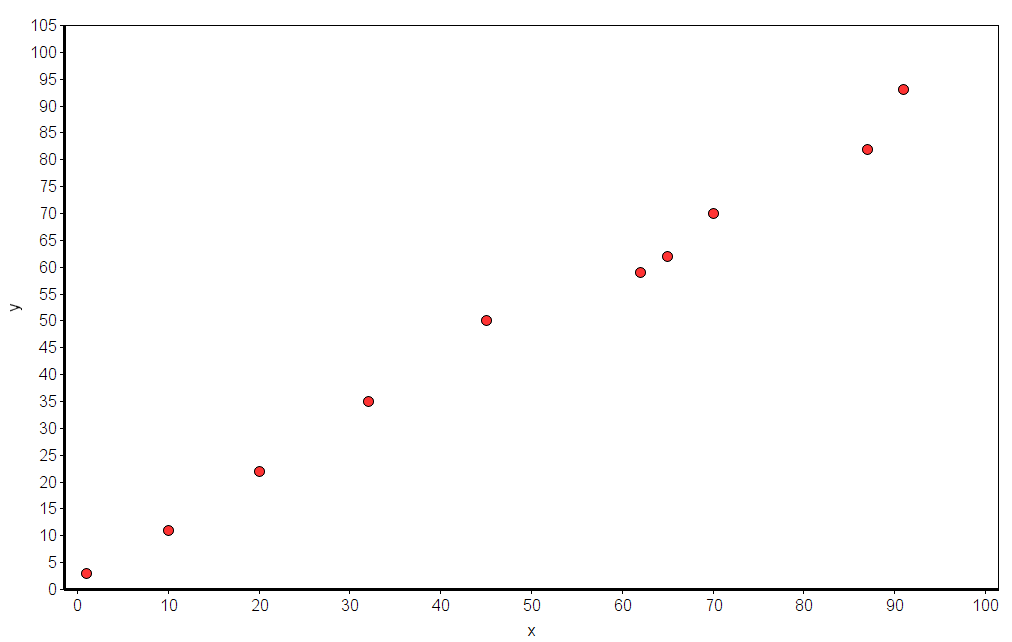
\includegraphics[scale=0.65]{images/compress2d.png}
	\caption{Beispielhafte Verteilung von Messwerten.}
	\label{img:compress2}
\end{figure}

\todo{Hier related work? Dann Festlegung}
Ein moderner Ansatz für diesen Zweck ist die Verwendung neuronaler Netze. Ein Autoencoder ist ein spezielles neuronales Netzwerk, welches für das Lernen einer komprimierten Darstellung von Daten verwendet wird. Das Konzept des Autoencoders reicht zwar bis in die 80er Jahre zurück, eine Methode zum Training tiefer Netze ist aber erst 2006 von Hinton \cite{dae2006} entwickelt worden. Um solche einen kompakteren Feature-Deskriptor zu erzeugen, soll ein Autoencoder verwendet werden. Ein mehrstufiger Autoencoder kann mit jeder Schicht einen kompakteren Deskriptor erzeugen und kodiert die gelernten Informationen in den Gewichten. Der Autoencoder bringt darüber hinaus den Vorteil mit sich, das seine Architektur bereits auf eine parallele Verarbeitung ausgelegt ist und nicht \enquote{extra} berücksichtigt werden muss.

\section{Feature Detektion und Deskription}
\label{extraction}

Für die weitere Verarbeitung der Features ist es erstrebenswert, dass ihre Darstellung möglichst kompakt ist. Deskriptoren werden als Vektoren von Zahlen kodiert, die abhängig vom Verfahren Informationen über einen Pixel und seine Nachbarschaft oder auch ein ganzes Bild enthalten. Je größer die Anzahl der Einträge eines Vektors, desto größer wird der Speicherbedarf und Rechenaufwand.
Die erste Stufe des vorgestellten Modells sieht daher die Komprimierung der Feature-Vektoren durch einen Autoencoder vor. Auf diese Weise kann ein initial recht umfangreicher Feature-Vektor aufgebaut werden: Jede Stufe des Autoencoders lernt dann eine kompaktere Darstellung des Feature-Vektors bis zu einer gewünschten Untergrenze.\newline
Da für die vorliegenden Bilddaten der HsH keine speziellen Annahmen getroffen werden können, ist nicht bekannt was für eine Art von Deskriptor gute Ergebnisse liefern kann. In der Literatur findet sich eine große Anzahl an Verfahren zur Detektion und Extraktion von Features für etliche Zwecke. Um einen Überblick zu geben, sollen einige Vertreter angeführt werden, um den Leser einzuführen.

\subsection{Detektoren}

Feature-Detektoren für Bilder sind in die Kategorien \textit{single-scale},\textit{multi-scale} und \textit{affine invariant} eingeteilt. Detektoren berücksichtigen im Allgemeinen Transformationen wie Rotationen oder Verschiebungen sowie Variationen in der Beleuchtung. Die \textit{multi-scale} Detektoren berücksichtigen zusätzlich Änderungen im Maßstab. Liegen also zwei Bilder vor, die das gleiche Objekt in unterschiedlicher Größe zeigen, werden die gleichen \textit{keypoints} gefunden. Da nicht die Annahme getroffen werden kann, dass die Objekte in den Daten der HsH im gleichen Maßstab vorliegen, liegt hier der Fokus auf \textit{multi-scale} Detektoren. Einige populäre Vertreter, die hierfür in Frage kommen, werden im folgenden vorgestellt.

\textbf{Laplacian-of-Gaussian} \todo{Under Construction. Hier oder Grundlagenkapitel? Dann auch Difference of Gaussians und HOG / SIFT zu den Deskriptoren} %Der Laplacian of Gaussians ist ein Detektor für Regionen. %\todo{Laplacian-of-Gaussian (LoG), a linear combination of second derivatives, is a common blob detector. Given an input image I(x, y), the scale space representation of the image defined by L(x, y,delta) is obtained by convolving the image by a variable scale Gaussian kernel G(x, y,delta) where FORMEL 

%For computing the Laplacian operator, the following formula is used FORMEL 

%This results in strong positive responses for dark blobs and strong negative responses for bright blobs of size root2delta. However, the operator response is strongly dependent on the relationship between the size of the blob structures in the image domain and the size of the smoothing Gaussian kernel. 

%The standard deviation of the Gaussian is used to control the scale by changing the amount of blurring. In order to automatically capture blobs of different size in the image domain, a multi-scale approach with automatic scale selection is proposed in [36] through searching for scale space extrema of the scale-normalized Laplacian operator. FORMEL. 

%Which can also detect points that are simultaneously local maxima/minima of delta normL(x, y, delta) with respect to both space and scale. The LoG operator is circularly symmetric; it is therefore naturally invariant to rotation. The LoG is well adapted to blob detection due to this circular symmetry property, but it also provides a good estimation of the characteristic scale for other local structures such as corners, edges, ridges and multi-junctions. 

%In this context, the LoG can be applied for finding the characteristic scale for a given image location or for directly detecting scale-invariant regions by searching for 3D (location + scale) extrema of the LoG function as illustrated in Fig. 6.

\textbf{Difference of Gaussians} Dieser Detektor ist eine von Lowe entwickelte Alternative zum Laplacian of Gaussians. Dieser Algorithmus ist zwar nicht genauso präzise, erreicht aber in kürzerer Zeit eine Annäherung die \enquote{gut genug} ist. Da die Bilder der verschiedenen Oktaven im \textit{scale space} (siehe Grundlagen) voneinander subtrahiert werden, ist hier keine Faltung notwendig. 


%\todo{In fact, the computation of LoG operators is time consuming. To accelerate the computation, Lowe [31] proposed an efficient algorithm based on local 3D extrema in the scale-space pyramid built with Difference-of-Gaussian(DoG) filters. This approach is used in the scale-invariant feature transform (SIFT) algorithm. In this context, the DoG gives a close approximation to the Laplacian-of-Gaussian (LoG) and it is used to efficiently detect stable features from scale-space extrema. The DoG function D(x, y, delta) can be computed without convolution by subtracting adjacent scale levels of a Gaussian pyramid separated by a factor k. FORMEL Feature types extracted by DoG can be classified in the same way as for the LoG operator. Also, the DoG region detector searches for 3D scale space extrema of the DoG function as shown in Fig. 7. The computation of LoG operators is time consuming. The common drawback of both the LoG and DoG representations is that the local maxima can also be detected in neighboring contours of straight edges, where the signal change is only in one direction, which make them less stable and more sensitive to noise or small changes [45].}

\subsection{Deskriptoren}

\todo{Das ist der aktuelle Stand. Hierher komplett HOG und SIFT verschieben (dadurch auch weniger Wiederholung..)? Dafür LBP und Spatial Envelope raus (Spatial Envelope scheidet ja im Grunde schon durch den Fokus auf die Objekterkennung aus, ist noch \enquote{über}).}

Hier werden einige ausgewählte Deskriptoren vorgestellt, die auf unterschiedliche Anwendungsfälle ausgelegt sind. Der \textit{Spatial Envelope} beurteilt beispielsweise die \enquote{Art} einer Szene, die Local Binary Patterns werden vorwiegend zur Gesichtserkennung verwendet. \newline

\textbf{Local Binary Patterns} Die Local Binary Patterns (LBP) kodieren eine Nachbarschaft eines Pixels, also einen lokalen Teil eines Bildes, indem der Pixel mit seinem Nachbarn verglichen wird. Klassisch wird hier einer $3 \times 3$ Matrix verwendet, sodass sich acht Werte und somit 256 mögliche Kodierungen ergeben.
Praktisch erzielt der Einsatz von LBP vor allem im Bereich der Gesichtserkennung und Erkennung von Nummernschildern gute Ergebnisse. Durch die kleine $3 \times 3$ Matrix werden gerade feine Details berücksichtigt, allerdings können dadurch keine makroskopischen Zusammenhänge berücksichtigt werden. Hierfür können auch größere Nachbarschaften gewählt werden, allerdings gehen dann die Details verloren.\newline 

\textbf{Spatial Envelope} In diesem Ansatz wird davon ausgegangen, dass Menschen eine Szene auch einordnen können, wenn diese in geringer Auflösung vorliegt. Der \textit{Spatial Envelope} beschreibt daher das Bild durch globale Features. Torralba und Olivia \cite{mts2001} haben mit dem  \textit{Spatial Envelope} ein Verfahren entwickelt, um die z.B. die Natürlichkeit oder Offenheit einen Szene zu beurteilen. Eine hohe Natürlichkeit weist zum Beispiel auf das Bild einer Landschaft hin: Hier kommen in der Regel kaum gerade vertikale und horizontale Linien vor, im Gegensatz zu Bildern, die von Menschen angefertigt wurden.\newline

\textbf{SIFT} Der 1999 von Lowe entwickelte SIFT-Deskriptor, ist der einer der häufigst genutzten für die Objekterkennung in Bildern. Der Deskriptor besitzt zwar keine affine Invarianz, in praktischen Anwendungen werden jedoch auch mit skalierten, rotierten und verschobenen Objekten gute Ergebnisse erzielt.
Der mathematische Hintergrund von SIFT wurde wurde bereits im Grundlagen behandelt. Mikolajczyk und Schmid \cite{idp2005} haben 2005 SIFT mit anderen Deskriptoren (u.a. shape context, komplexe Filter, gradient location and orientation histogram, moment invariants, ...) verglichen und kamen zu dem Ergebnis, dass SIFT sehr gut hinsichtlich der Präzison abschneidet. Die Konstruktion des Deskriptors ist allerdings aufwändig und die Beschreibung erfordert einen Feature-Vektor mit 128 Komponenten.\newline

\subsection{Features in dieser Arbeit}

In dieser Arbeit wird das Gruppieren der Bilder durch eine Objekterkennung realisiert. Hiermit eignen sich vor allem \textit{multi-scale} Detektoren. Bei der Auswahl des Deskriptors scheint SIFT, aufgrund der praktischen Erfolge, naheliegend. Die Frage ist, ob bei der Verwendung von SIFT eine weitere Komprimierung noch sinnhaft ist. Die Neuronenanzahl der Schichten eines Stacked Autoencoders nehmen strikt ab, um die Komprimierung zu erreichen. Dies führt dazu, dass zwischen \textit{Input} und dem folgenden \textit{Hidden Layer} maximal $128 \times 127 = 16256$ Verbindungen existieren können. Zhao \cite{aed2016} hat aus diesem Grund einen anderen Ansatz gewählt: Die \textit{keypoints} werden zunächst, wie bei SIFT, durch den DoG-Operator ermittelt. Anschließend wird ein großer Deskriptor aus den Gradienten der Nachbarschaften um die \textit{keypoints} erzeugt, der dann als Eingabe für den Autoencoder dient. Dieser komprimiert den Vektor auf 36 Komponenten. Gegenüber SIFT ist diese Darstellung ca. $3,5$ mal kleiner, was einen nicht unerheblichen Teil, gerade wegen der großen Menge an Features, ausmacht.\newline
Aus diesem Grund sollen zwei Varianten in der Konzeption verfolgt werden: Zum einen die Verwendung von SIFT-Features und zum anderen das Erzeugen des Deskriptors nach Zhao durch einen Autoencoder. Durch die Kompaktheit des Letzteren ist zu erwarten, dass der Clustering-Vorgang bei diesem um ein vielfaches schneller abgeschlossen ist. Dabei war die Qualität der Ergebnisse von Bildervergleichen in Zhaos Test sehr ähnlich. Ob dies auch für den Bag of Visual Words der Fall ist, soll ein Experiment zeigen.